%Packages are included below, these are akin to libraries in other programming languages. As far as I can tell, there is no reason to reduce the number of packages included in a document. It might compile faster, but overleaf compiles fast so this should not be an issue.
\documentclass[english, 11pt, letterpaper]{report} %tells the compiler that this is a 'report' style document, and the main font size.

\usepackage[utf8]{inputenc} %inclusion of this is optional, overleaf includes it in its compiler so it is not necessary, it may be necessary for other compilers.
\usepackage[english]{babel} %this does a few things eg allowing dates to be made by the compiler. probably best not to get rid of it
\usepackage{graphicx} %this allows graphics to be put in easily
\usepackage{float}%this allows you to put them in good places
% \usepackage[version=4]{mhchem} %this is good for chemical reactions
\usepackage{amsmath} %maths package
\usepackage{amssymb} %symbol package
\usepackage{textcomp,gensymb} %more symbols (eg \degree)
\usepackage{appendix} %self explanatory
\usepackage{colortbl} %good for colouring in cells on a table
\usepackage{rotating} %allows you to rotate graphics
\usepackage{bm} %helps bold things
\usepackage{multirow} %for tables
\usepackage{longtable} %for long tables
\usepackage{booktabs} %more tables
\usepackage{pdfpages} %allows PDFs to be included in document (good if you want to include a pdf in an appendix eg)
\usepackage{caption} %allows captions for graphics
\usepackage[nottoc]{tocbibind} %adds the bibliography to the table of contents
\usepackage{subcaption} %allows subcaption for multiple images in one graphic

\PassOptionsToPackage{hyphens}{url}\usepackage{hyperref}
\usepackage{hyperref} %this is great for putting hyperreferences in the document.
\usepackage[table]{xcolor} %more colouring of tables
\definecolor{Gray}{gray}{0.9} %this defines a colour to be used and gives it a name. This is a colour called 'Gray' it is 'gray' with transparency 0.9
\hypersetup{colorlinks=false} %this stops links being colourful, which makes a report look less professional I believe.


\usepackage[letterpaper, top=0.5in, bottom = 0.5in, right = 0.5in, left=0.5in]{geometry} %this describes the layout of the document and the margins etc.
% \usepackage{setspace} %allows the use of '\doublespace' to set line spacing
%\doublespacing %self explanatory
\renewcommand{\baselinestretch}{1.5}

% Single spaces after periods.
\frenchspacing

% Font to Helvetica.
\usepackage{helvet}
\renewcommand{\familydefault}{\sfdefault}

% Specific command for the KRAS gene.
\newcommand{\KRAS}{\emph{KRAS}}
% Specific command for the KRAS protein.
\newcommand{\kras}{K-RAS}

\usepackage[T1]{fontenc}
\usepackage{titlesec, blindtext, color}
\definecolor{gray75}{gray}{0.75}
\newcommand{\hsp}{\hspace{20pt}}

% Styling of Chapter and Section titles.
\titleformat{\chapter}[hang]{\LARGE\bfseries}{\thechapter\hsp\textcolor{gray75}{|}\hsp}{0pt}{\LARGE\bfseries}
\titleformat{\section}[hang]{\Large\bfseries}{\thechapter\hsp\textcolor{gray75}{|}\hsp}{0pt}{\Large\bfseries}
\titleformat{\subsection}[hang]{\large\bfseries}{\thechapter\hsp\textcolor{gray75}{|}\hsp}{0pt}{\large\bfseries}
\titleformat{\subsubsection}[hang]{\normalsize\itshape}{\thechapter\hsp\textcolor{gray75}{|}\hsp}{0pt}{\normalsize\itshape}

% Use "References" instead of "Bibliography".
\AtBeginDocument{\renewcommand{\bibname}{References}}

\begin{document} % you have to do this to start the document

%%%%%%%%%%%%%%%%%%%%%%%%%%%%%%%%%%%%%%%%%%%
%For a long report such as a thesis, I would recommend thinking like programming, that is, have a short 'main' and long programs (or chapters in this case) this allows you to access each chapter easily and see the layout of the document easily.
%
%using \input{} basically puts the code specified in the argument (between the braces) into the body of the code in main
%%%%%%%%%%%%%%%%%%%%%%%%%%%%%%%%%%%%%%%%%%%

% The entire thesis is generated by the commands below, referencing the other files in this directory.

%%%%%%%%%%%%%%%%%%%%%%%%%%%%%%%%%%%%%%%%%%%
% Preamble
%%%%%%%%%%%%%%%%%%%%%%%%%%%%%%%%%%%%%%%%%%%

\begin{titlepage}
    \begin{center}
        \vspace*{2cm}
        % this title page can be played around with to better serve your project. the necessary parts to include are the TITLE at the top, the BLURB about the thesis presented etc. Name, faculty member, date, type of engineering...
        \LARGE
        \vspace{3cm}
        \textbf{Studying tissue-specificity of cancer in the context of \KRAS{}}

        \vfill
 
        \Large
        \textbf{Joshua H. Cook} \\
        \vspace{1cm}
        3rd year Ph.D. candidate \\
        Biological and Biomedical Sciences at Harvard Medical School \\
        email: jhcook@g.harvard.edu \\
        (Initial DAC meeting) \\
        Faculty Advisors: Kevin M. Haigis and Peter J. Park \\
        DAC Committee: Shamil Sunyaev (Chair), William Hahn, Matthew Meyerson \\
        June 10, 2020 from 3pm to 5pm \\
        The meeting will be held virtually over Zoom.\\
        \vspace{2cm}
 
    \end{center}
\end{titlepage}


\pagenumbering{roman} %Roman numbering is recommended until the body

\tableofcontents 

% \listoffigures 

% \listoftables 

\chapter*{Abstract}
\normalsize

An abstract that provides a brief outline of the report.
 

\pagenumbering{arabic} %back to Arabic numbering for the rest

%%%%%%%%%%%%%%%%%%%%%%%%%%%%%%%%%%%%%%%%%%%
% Chapters
%%%%%%%%%%%%%%%%%%%%%%%%%%%%%%%%%%%%%%%%%%%

\chapter{Introduction}

\subsection*{The tissue-specific paradigm of cancer biology.}

While many think of cancer as the destruction of cellular regulatory mechanisms resulting in an unregulated, anarchical system, advances in cancer genetics have revealed it to be a highly organized and complex disease.
As such, specific alterations to the normal cell are required for transformation, resulting in these changes displaying strong tissue-specificity.
The phenomenon of tissue-specificity of cancer drivers has been extensively reviewed elsewhere \cite{Sieber2005TissueCancers., Schneider2017, Haigis2019}, but the basic principle is that the effect of a disruption (e.g. a single nucleotide substitution, copy number alteration, dysregulated gene expression, chromosomal rearrangement, etc.) is determined by the preexisting cellular and tissue signaling environments.
As a result, the identification of a panacea for cancer is unlikely, and, instead, advances in therapeutics will rely upon improved precision medicine where each tumor is treated based on its unique properties.

The goal of the research proposed herein is to study the phenomenon of tissue-specificity via two strategies.
In the first, we will study the oncogene \KRAS{} in various tissues, characterizing its genetic interactions in different cancers (Aim 1) and identifying underlying properties of tissues that determine the potency of its oncogenic mutations (Aim 2).
From these analyses, we will have a better understanding of how the interactions of the same gene are dependent upon the broader tissue-specific context.
The second strategy we will employ to understand tissue-specificity of oncogenesis is to analyze the effects of a change to the broader cellular context on the mechanisms capable of driving cancer.
This will be accomplished by identifying the impacts of disrupted epigenetic modifications from dysregulated polycomb repressive complex 2 (PRC2) on a cancer's oncogenic mutations, genetic interactions, and genetic dependencies (Aim 3).


\subsection*{\KRAS{} is a tissue-specific oncogene.}

\kras{} (encoded by the \KRAS{} gene) is a member of the Ras family of highly homologous, small GTPases, ubiquitously expressed in humans \cite{Barbacid1987, Prior2012}. 
They operate as GTP-regulated signaling hubs, relaying extracellular signals to key intracellular functions such as growth, proliferation, metabolism, and motility. 
When bound to GTP, \kras{} activates its downstream effectors via protein-protein interactions until it is deactivated by hydrolyzing the GTP to GDP with assistance from GTPase-activating proteins (GAPs). 
The release of GDP, facilitated by guanine nucleotide exchange factors (GEFs), allows \kras{} to again bind a GTP molecule, returning to its active state \cite{Barbacid1987, Johnson2017}. 
Mutations of \KRAS{} that result in a net increase of the cellular concentration of GTP-bound \kras{} are frequently initiating events in cancer \cite{Kanda2012, Zhang2014a, Li2018, Prior2020TheCancer}, though are specifically enriched in colorectal adenocarcinoma (COAD, mutated in about 50\% of tumors), lung adenocarcinoma (LUAD, 30\%), multiple myeloma (MM, 20\%), and pancreatic adenocarcinoma (PAAD, 90\%) \cite{Prior2020TheCancer}.
In contrast, \KRAS{} is very rarely mutated in other cancer types, resulting in two groups of tissues: \KRAS{}-sensitive and \KRAS{}-insensitive.

\textbf{In Aim 1, we propose to study the different oncogenic variants (or "alleles") of \KRAS{} in \KRAS{}-sensitive tissues as a method through which to investigate tissue-specific genetic interactions of an oncogene.}
First we will study the ability of various mutational processes to cause each allele as a means to explain the allelic diversity across cancer types.
Then we will identify comutation interactions and genetic dependencies between the \KRAS{} alleles and other genes to measure each variant's distinct effect on cancer progression.
These results will highlight the necessity to study cancer drivers at the tissue- and allele-level in order to fully describe their oncogenic properties.

\textbf{Aim 2 proposes to reveal differences in \KRAS{}-sensitive and insensitive tissues that explain the vast disparity in mutational frequencies across cancer types.}
Similar to Aim 1, we will begin by estimating the extent to which active mutational processes contribute to the rate of \KRAS{} mutation.
We will then attempt to model the permissivity of a tissue to mutant \KRAS{} on the basal proteomic and phosphoproteomic state.
Finally, the rare instances of \KRAS{}-insensitive cancers with \KRAS{} mutations will be analyzed to determine if and how they became \KRAS{}-sensitive.
These studies will provide insight into the mechanisms that determine the tissue-specificity of \KRAS{}-driven cancer.


\subsection*{Dysregulated PRC2 augments the epigenetic state of a cell.}

% General information.
PRC2 is a protein complex that suppresses gene expression by mono-, bi-, and trimethylating lysine 27 of histone H3 (H3K27).
It is essential for human development, modulating and maintaining the epigenetics of cells as they grow and differentiate.
The complex is composed of four core subunits, EZH2 (or the homolog EZH1), SUZ12, EED, and RBBP4/7 (also known as RBAP46/48), and two subtypes, PRC2.1 and  PRC2.2, have been identified as the association of the core subunits with groups of other proteins.
These auxiliary subunits are thought to regulate the enzymatic activity of EZH1/2 and help recruit the complex to different locations on the chromosomes \cite{VanMierlo2019a, Laugesen2019a}.
Exactly how PRC2 is recruited to specific chromosomal locations is still an activate area of research, though there is a known association with unmethylated CpG islands  \cite{Ku2008, Tanay2007HyperconservedSites., Mendenhall2010GC-richCells., Lynch2012AnRecruitment.}.
Additional studies suggest that transcription factors, non-coding RNA, and histone modifications \cite{Laugesen2019a}, including its own product, the methylation of H3K27, influence the localization of PRC2.

% As a system for understanding changes in context (Aim 3)
Previous studies have revealed instances where the behaviour of oncogenes can change in response to epigenetic changes from PRC2 dysregulation \cite{Kim2015SWI/SNF-mutantEZH2., Fillmore2015EZH2Inhibitors., Serresi2016PolycombCancer., Serresi2018Ezh2Vulnerabilities., Chen2018TargetingMedicine.}.
For example, inhibition of EZH2 in NSCLC cell lines with either an \emph{EGFR} or \emph{SMARCA4} mutation were more susceptible to inhibition of topoisomerase II (TopoII).
If both of these genes were wild-type (WT), however, EZH2 inhibition resulted in upregulated \emph{SMARCA4}, mediating resistance to TopoII inhibition \cite{Fillmore2015EZH2Inhibitors.}.
These studies suggest that the epigenetic changes due to altered PRC2 activity cause substantial alterations to cellular signaling, augmenting the oncogenic potential of some genes.

\textbf{Therefore, in Aim 3, we propose to study the impact of dysregulated PRC2 as a mechanism for analyzing the consequences of a change to the signaling environment on the tissue-specificity of oncogenes.}
We will start by identifying genes that experience different rates of mutation or demonstrate distinct comutation interactions under abnormal PRC2 activity in human tumor samples.
In addition, we will identify genes with differing levels of dependency in cancer cell lines with dysregulated PRC2.
These analyses to characterize changes to the drivers of cancer under an altered epigenetic state will model the impact of the cellular context on oncogene fitness.


\chapter{Experimental Design}

\section*{Aim 1. A statement about what Aim 1 is.}

\subsection*{Rationale}

\subsection*{Aim 1.1. A statement about what Aim 1.1 is.}

\subsubsection*{Approach}

\subsubsection*{Pitfalls and alternative approaches}

\subsubsection*{Preliminary data}

\subsection*{Aim 1.2. A statement about what Aim 1.2 is.}

\subsubsection*{Approach}

\subsubsection*{Pitfalls and alternative approaches}

\subsubsection*{Preliminary data}

\subsection*{Aim 1.3. A statement about what Aim 1.3 is.}

\subsubsection*{Approach}

\subsubsection*{Pitfalls and alternative approaches}

\subsubsection*{Preliminary data}



\section{Aim 2. Elucidate the characteristics that determine sensitivity to oncogenic \KRAS{} mutations.}

\subsection*{Rationale}

Though \KRAS{} is estimated to be mutated in 10\%-14\% \cite{Bailey2018, Prior2020TheCancer} of all cancer, only a few cancer types frequently have oncogenic \KRAS{} mutations.
One explanation for this phenomenon is that the actual mutational event is less likely to occur in some tissues compared to others due to differences in mutagenic processes.
However, this is unlikely because neighboring tissues often demonstrate drastically different rates of \KRAS{} mutation.
One striking example is how 32\% of lung adenocarcinoma, but only 4\% of small cell lung cancer tumors have a \KRAS{} mutation \cite{Bailey2018, Prior2020TheCancer}.
Additionally, experimental evidence has demonstrated that even the forced expression of mutant \kras{} does not induce a hyperproliferative phenotype in all tissues \cite{Ray2011EpithelialModel,  Parikh2012MouseResponses}.
Instead, we hypothesize that the basal state of a tissue, including the existing signaling architecture, determines its sensitivity to \KRAS{} hyperactivation.
Therefore, I aim to identify properties of tissues that determine their sensitivity to \KRAS{} oncogenesis.

%%%%%%%%%%%%%%%%%%%%%%%%%%%%%%%%%%%%%%%%%%%
% Aim 2.1
%%%%%%%%%%%%%%%%%%%%%%%%%%%%%%%%%%%%%%%%%%%

\subsection*{Aim 2.1. Determine the extent to which mutational processes affects the frequency of \KRAS{} mutations across the cancers.}

\subsubsection*{Approach}

As mentioned previously, one explanation for the vast variation in \KRAS{} mutational frequency amongst different cancer types is that the causative mutations are more common in some tissues than others.

Mutational signatures will be used to assess the ability of various cancer types to obtain an oncogenic \KRAS{} mutation.
This will be accomplished via similar means as explained in Aim 1.1: by calculating the expected frequency of \KRAS{} mutations according to the genome-wide frequency of mutations in identical trinucleotide contexts.
However, instead of normalizing the values to report the probability of each allele to occur in each tumor sample, the values will be normalized to the total number of mutations in the tumor sample.
Thus, they will be comparable across cancer samples as a measure of the ability to gain a \KRAS{} mutation.

In addition, I will explore the use of count-based statistical models to extract additional information not available in aggregated statistics.
To begin, a logistic model will be fit to the number of mutations that could cause an activating \KRAS{} mutation and the total number of mutations to predict whether the tumor sample had a \KRAS{} mutation.
The coefficients of the fit model will be estimates of the impact of the types of mutations found in each sample on the probability of having a \KRAS{} mutation.
Additional models will be fit with fewer (e.g. just the total number of mutations) or additional (e.g. the mutation of other oncogenes such as \emph{BRAF} or \emph{EGFR}, stage of cancer, etc.) covariates to estimate the predictive power of the number of mutations that could create an oncogenic \KRAS{} allele taking into account other factors.
Additional models that include random effects for the tissue of origin or use a mixture-distribution to model different underlying rates of mutation can be compared to the logistic models.

Because there is experimental evidence that the tissue-of-origin determines the effect of hyperactive \kras{}, I expect that the number of mutations that could cause a \KRAS{} mutation will have little predictive power on whether a tumor sample has a \KRAS{} mutation.
Still, this analysis presents a rigorous statistical examination of this potential explanation.

\subsubsection*{Pitfalls and alternative approaches}

The proposed methods are limited in similar ways as mentioned in Aim 1.1.
Namely, this analysis will continue to assume that mutational forces act uniformly across the genome.

An additional limiting factor of the analysis will be the sparsity of \KRAS{} mutants in tumors from \KRAS{}-insensitive tissues.
This will limit the number of cancer types that can be studied as only those with a sufficient number of \KRAS{} mutants can be fit with the logistic models.

\subsubsection*{Preliminary data}

Currently, I have collected the sequencing data of about 42,000 tumor samples from 32 different tissues of origin.
Of this data set, 13,652 samples have targeted sequencing data and the remaining 28,321 samples were either whole genome or exome sequenced (WG/ES).
These cancers have been anatomically organized using the OncoTree graph from Memorial Sloan Kettering (Figure \ref{fig:oncotree}).

\begin{figure}[t!]
\centering
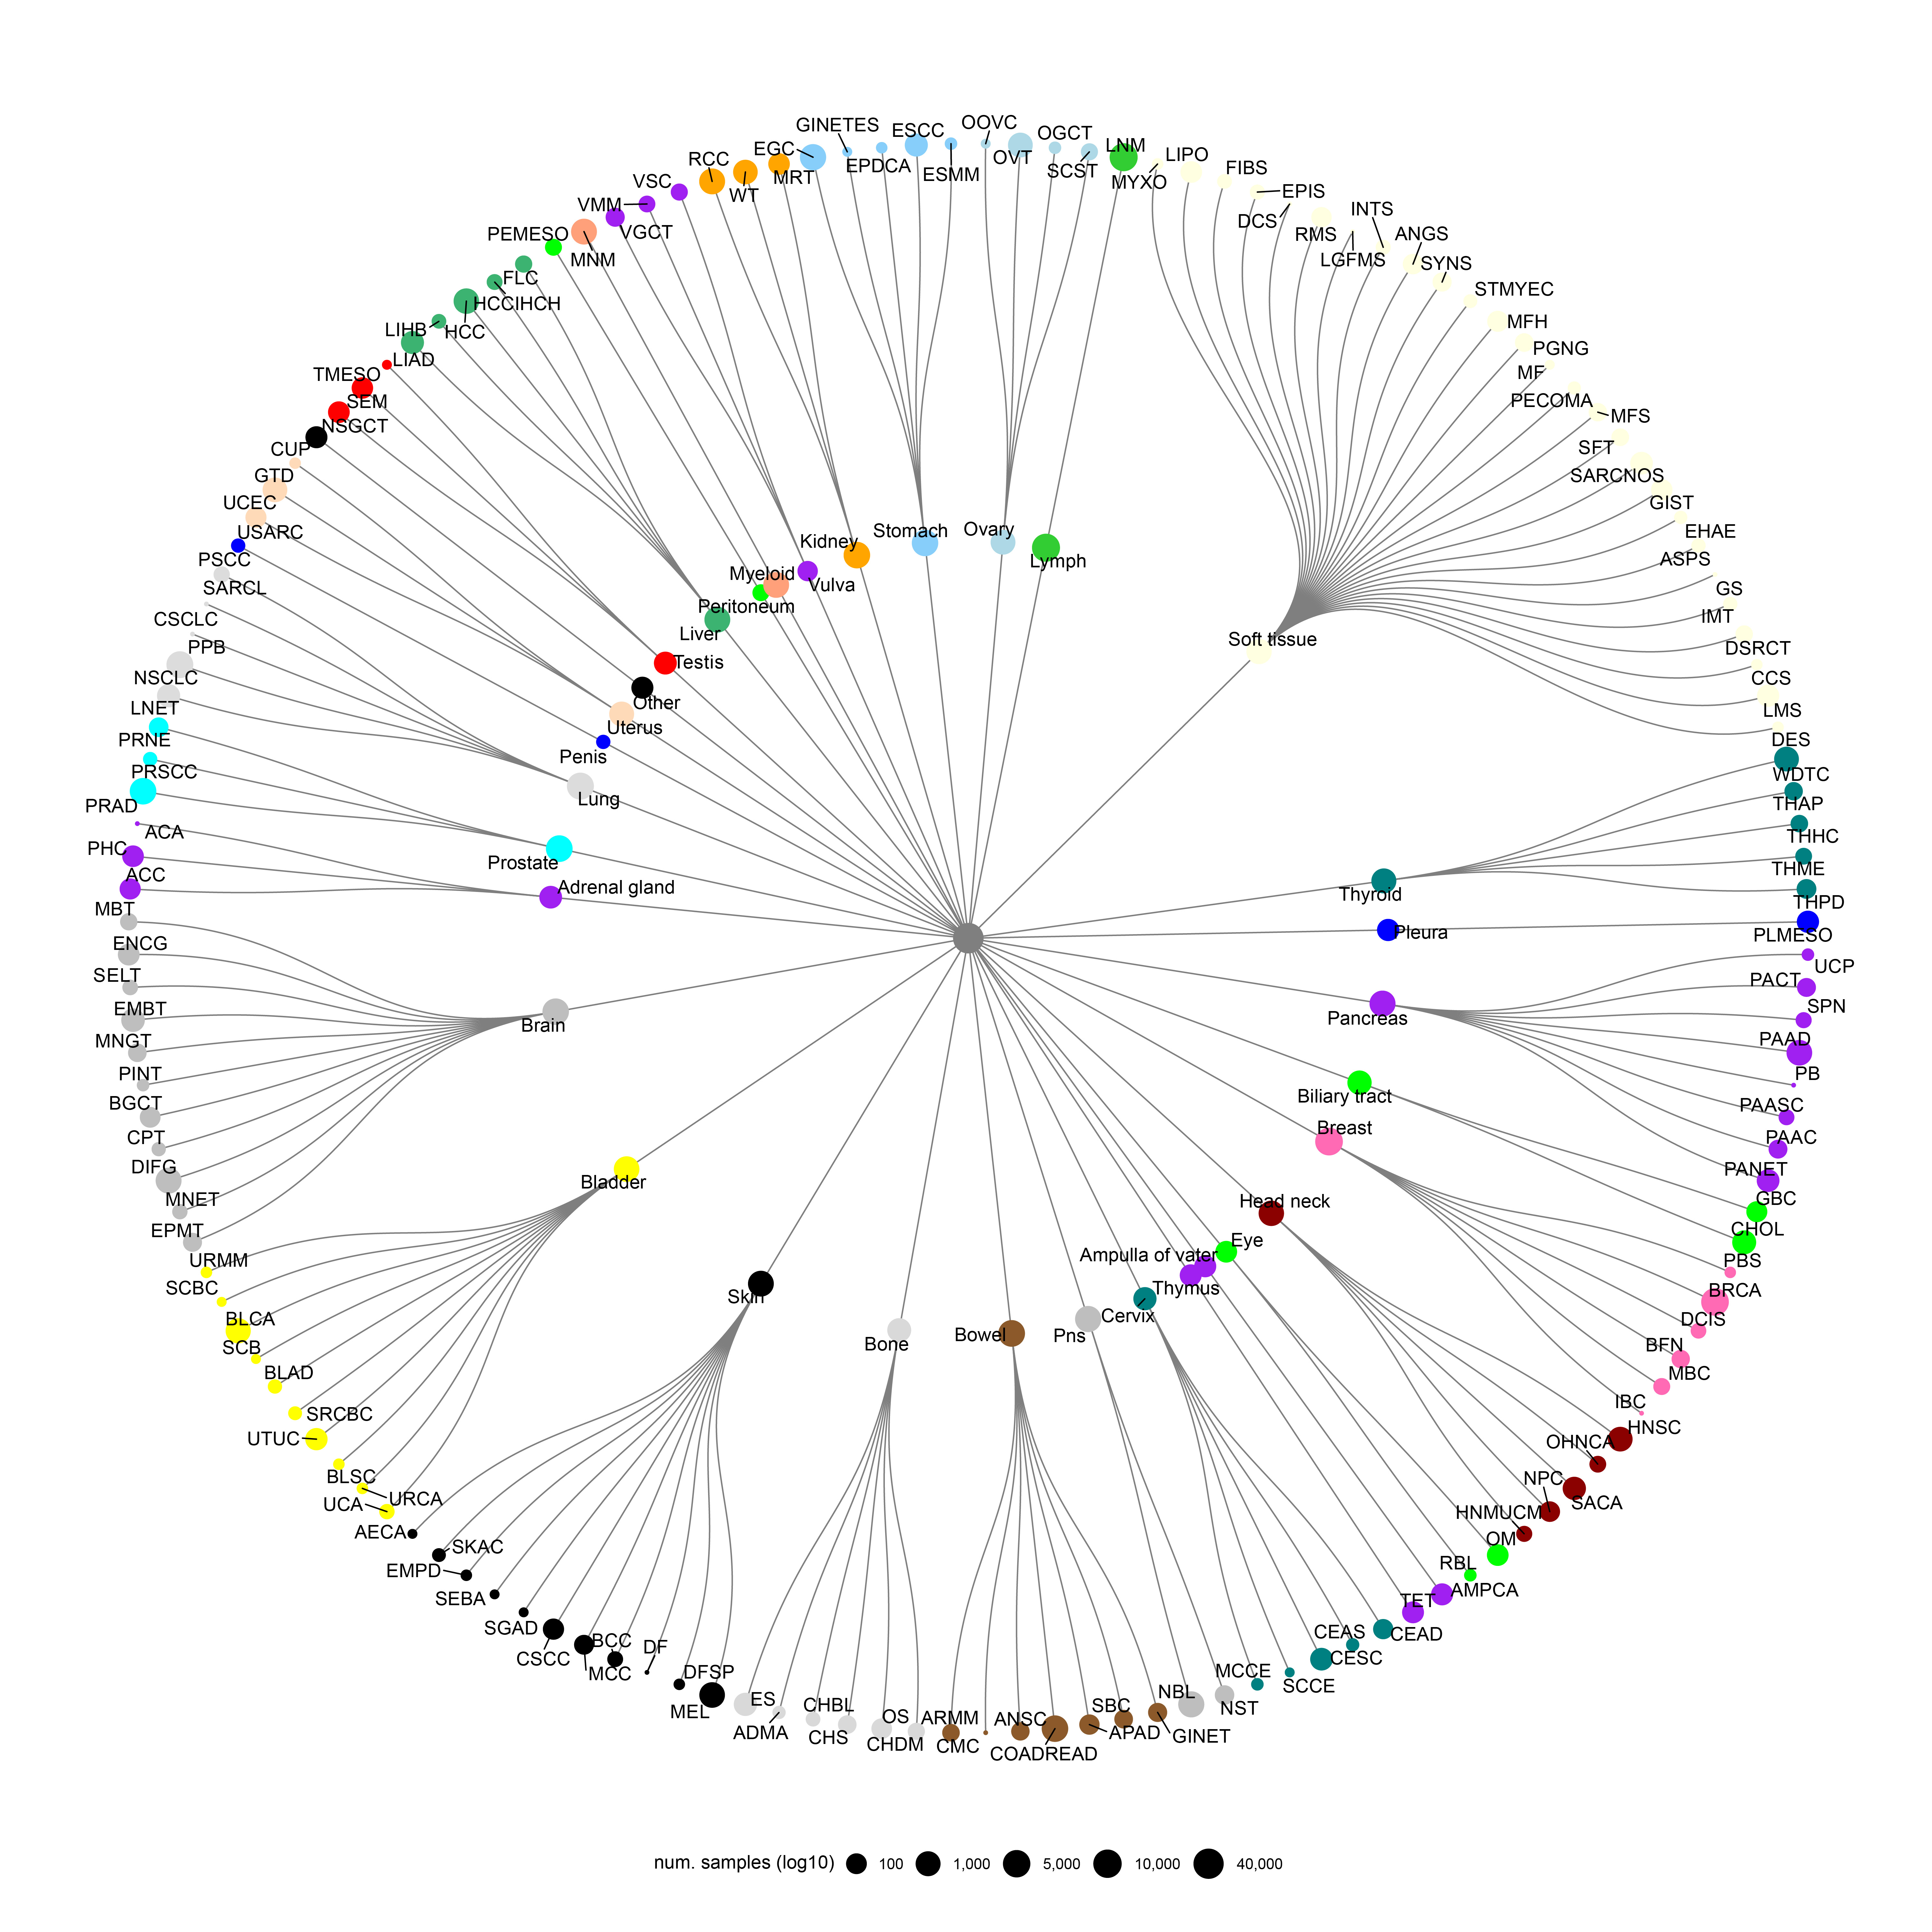
\includegraphics[width=180mm]{figures/aim2/oncotree_figure.jpg}
\caption{
    \textbf{The cancer samples were organized according to their anatomical relationships using the OncoTree.}
    Each layer from the middle represents a sub-location of the parent node.
    Nodes are colored by the parent organ and the size is related to the number of cancer samples that have been collected.
}
\label{fig:oncotree}
\end{figure}

As stated above, the number of \KRAS{} mutations will be a major determinant for whether mutation information from a cancer type can be analyzed as described.
Thus far, the \KRAS{}-insensitive tissues with the most number of samples with WG/ES data and an oncogenic \KRAS{} mutation include hepatocellular carcinoma, bladder urothelial carcinoma, cholangiocarcinoma, and esophagogastric adenocarcinoma (Figure \ref{fig:num-samples-kras-resistant}).

\begin{figure}[t!]
\centering
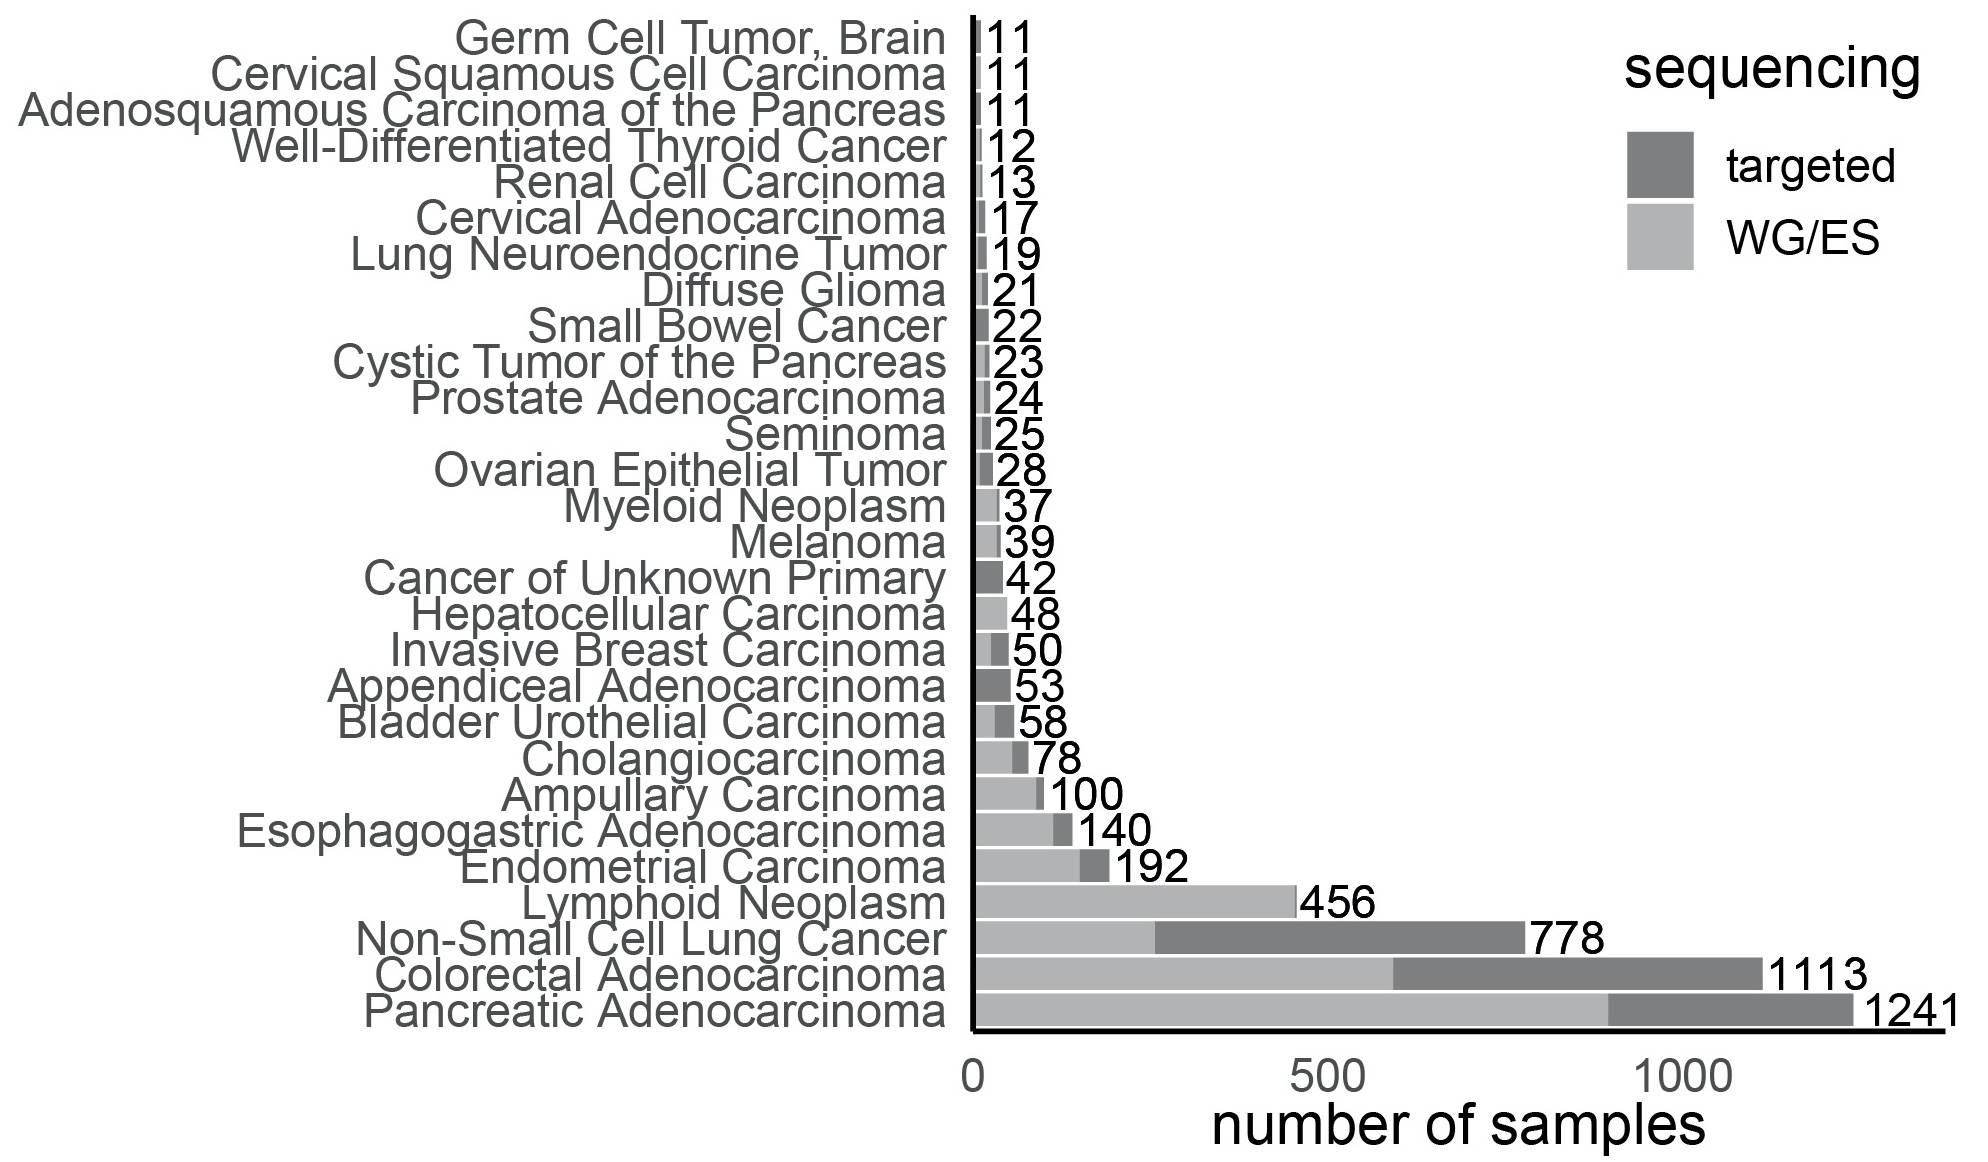
\includegraphics[width=120mm]{figures/aim2/kras-mutations-from-insensitive-tissues.jpg}
\caption{
    \textbf{The number of targeted sequenced and whole genome or exome sequenced (WG/ES) samples with \KRAS{} mutations.}
    Each cancer type (row) is annotated with the total number of samples with a \KRAS{} mutation.
}
\label{fig:num-samples-kras-resistant}
\end{figure}

%%%%%%%%%%%%%%%%%%%%%%%%%%%%%%%%%%%%%%%%%%%
% Aim 2.2
%%%%%%%%%%%%%%%%%%%%%%%%%%%%%%%%%%%%%%%%%%%

\subsection*{Aim 2.2. Model \KRAS{} sensitivity on the basal signaling of tissue.}

\subsubsection*{Approach}

Our hypothesis is that the structure of the ordinary signaling networks in a tissue determines its susceptibility to transformation by hyperactive \kras{} signaling.
Thus, I will use tandem-mass-tagged (TMT)-labeled \cite{Thompson2003} proteomic and phosphoproteomic data from \moKRAS{}\textsuperscript{WT/WT} mice collected by Dr. Olesja Popow to identify distinctions between sensitive and insensitive tissues.
The following organs were collected: colon, lung, pancreas, spleen (the "\KRAS{}-sensitive" tissues), heart, kidney, liver, skeletal muscle, and small intestine (the "\KRAS{}-insensitive" tissue).
The goal is to generate hypotheses that we could ultimately test in a mouse by pharmacologically or genetically modifying the insensitive tissue to make it sensitive to \KRAS{} mutation.

As before, I will model on whether or not the tissue is sensitive to \KRAS{} mutation. 
The amount of each protein, the amount of phosphorylation of each protein, the level of phosphorylation relative to the total amount of each protein, and ratios of different phosphorylations on the same protein can be used as input values.

Unless directly addressed, the high dimensionality of the data will cause the model to overfit.
As such, three strategies will be tested.
First, proteins that are involved in key signaling pathways (such as Wnt regulation, the MAPK pathway, or cell cycle regulation) will be selected.
Second, regularization or stepwise model selection algorithms will be used to reduce the number of predictors to just those with the most explanatory value by penalizing model complexity.
Third, latent-variable models such as partial least squares, principal component regression, or factor analysis will be tested.
These groups of methods provide a comprehensive comparative analysis of the many potentially explanatory models for the data.

\subsubsection*{Pitfalls and alternative approaches}

One limiting factor of the analysis will be the relatively few data points collected.
Twelve mice total were sacrificed, but, to increase the amount of protein for detection by mass spectrometry (MS) and reduce variation between samples, four (two females and two males) were pooled for each set of TMT-labeling.
Therefore, there are only 3 data points per protein per tissue.

The approach outlined above uses only linear models, though there are many non-linear models that could be used to identify differences between the two groups of tissues, such as support vector machines and random forest classifiers.
There are two primary reasons why I propose the use of linear models for the present study.
The first is that I believe that coefficients for the linear methods are more interpretable than the parameters used by non-linear methods.
The second is that the nonlinear methods have hyperparameters that must be tuned to prevent overfitting.
With such few data points, common methods such as cross-validation are not as effective.

A potential pitfall for this analysis is that \KRAS{} may not drive cancer via the same mechanism in all \KRAS{} sensitive tissues.
Conversely, the same may be true for how insensitive tissues stifle oncogenic \kras{} signaling.
Therefore, we will also build models using subsets of the tissues.
Subsets could include comparing a single sensitive tissue to all of the insensitive tissues, or comparing tissues of similar function but different sensitivity to \KRAS{} (such as the colon and the small intestine).

% These are mice and not humans. Tie in human information in the next sub-aim

\subsubsection*{Preliminary data}

As mentioned above, the proteomics and phosphoproteomics data have been collected for three groups of four mice.
Unsurprisingly, a preliminary exploratory analysis indicated that the strongest similarities are between samples is by organ.
When the dimensionality of the protein-space was reduced by PCA, plotting the t-SNE of the new dimensions demonstrated that the samples from the same organ clustered together (Figure \ref{fig:proteomics-eda}a, b).
Additionally, using a Student's \emph{t-test} to find the proteins that most clearly distinguished between the sensitive and insensitive tissues instead identified proteins with high tissue-specific expression (Figure \ref{fig:proteomics-eda}c).
These two precursory analyses demonstrate that organ-specific expression will present a major difficulty in finding relevant distinctions between the proteomics of sensitive and insensitive tissues.

\begin{figure}[ht]
\centering
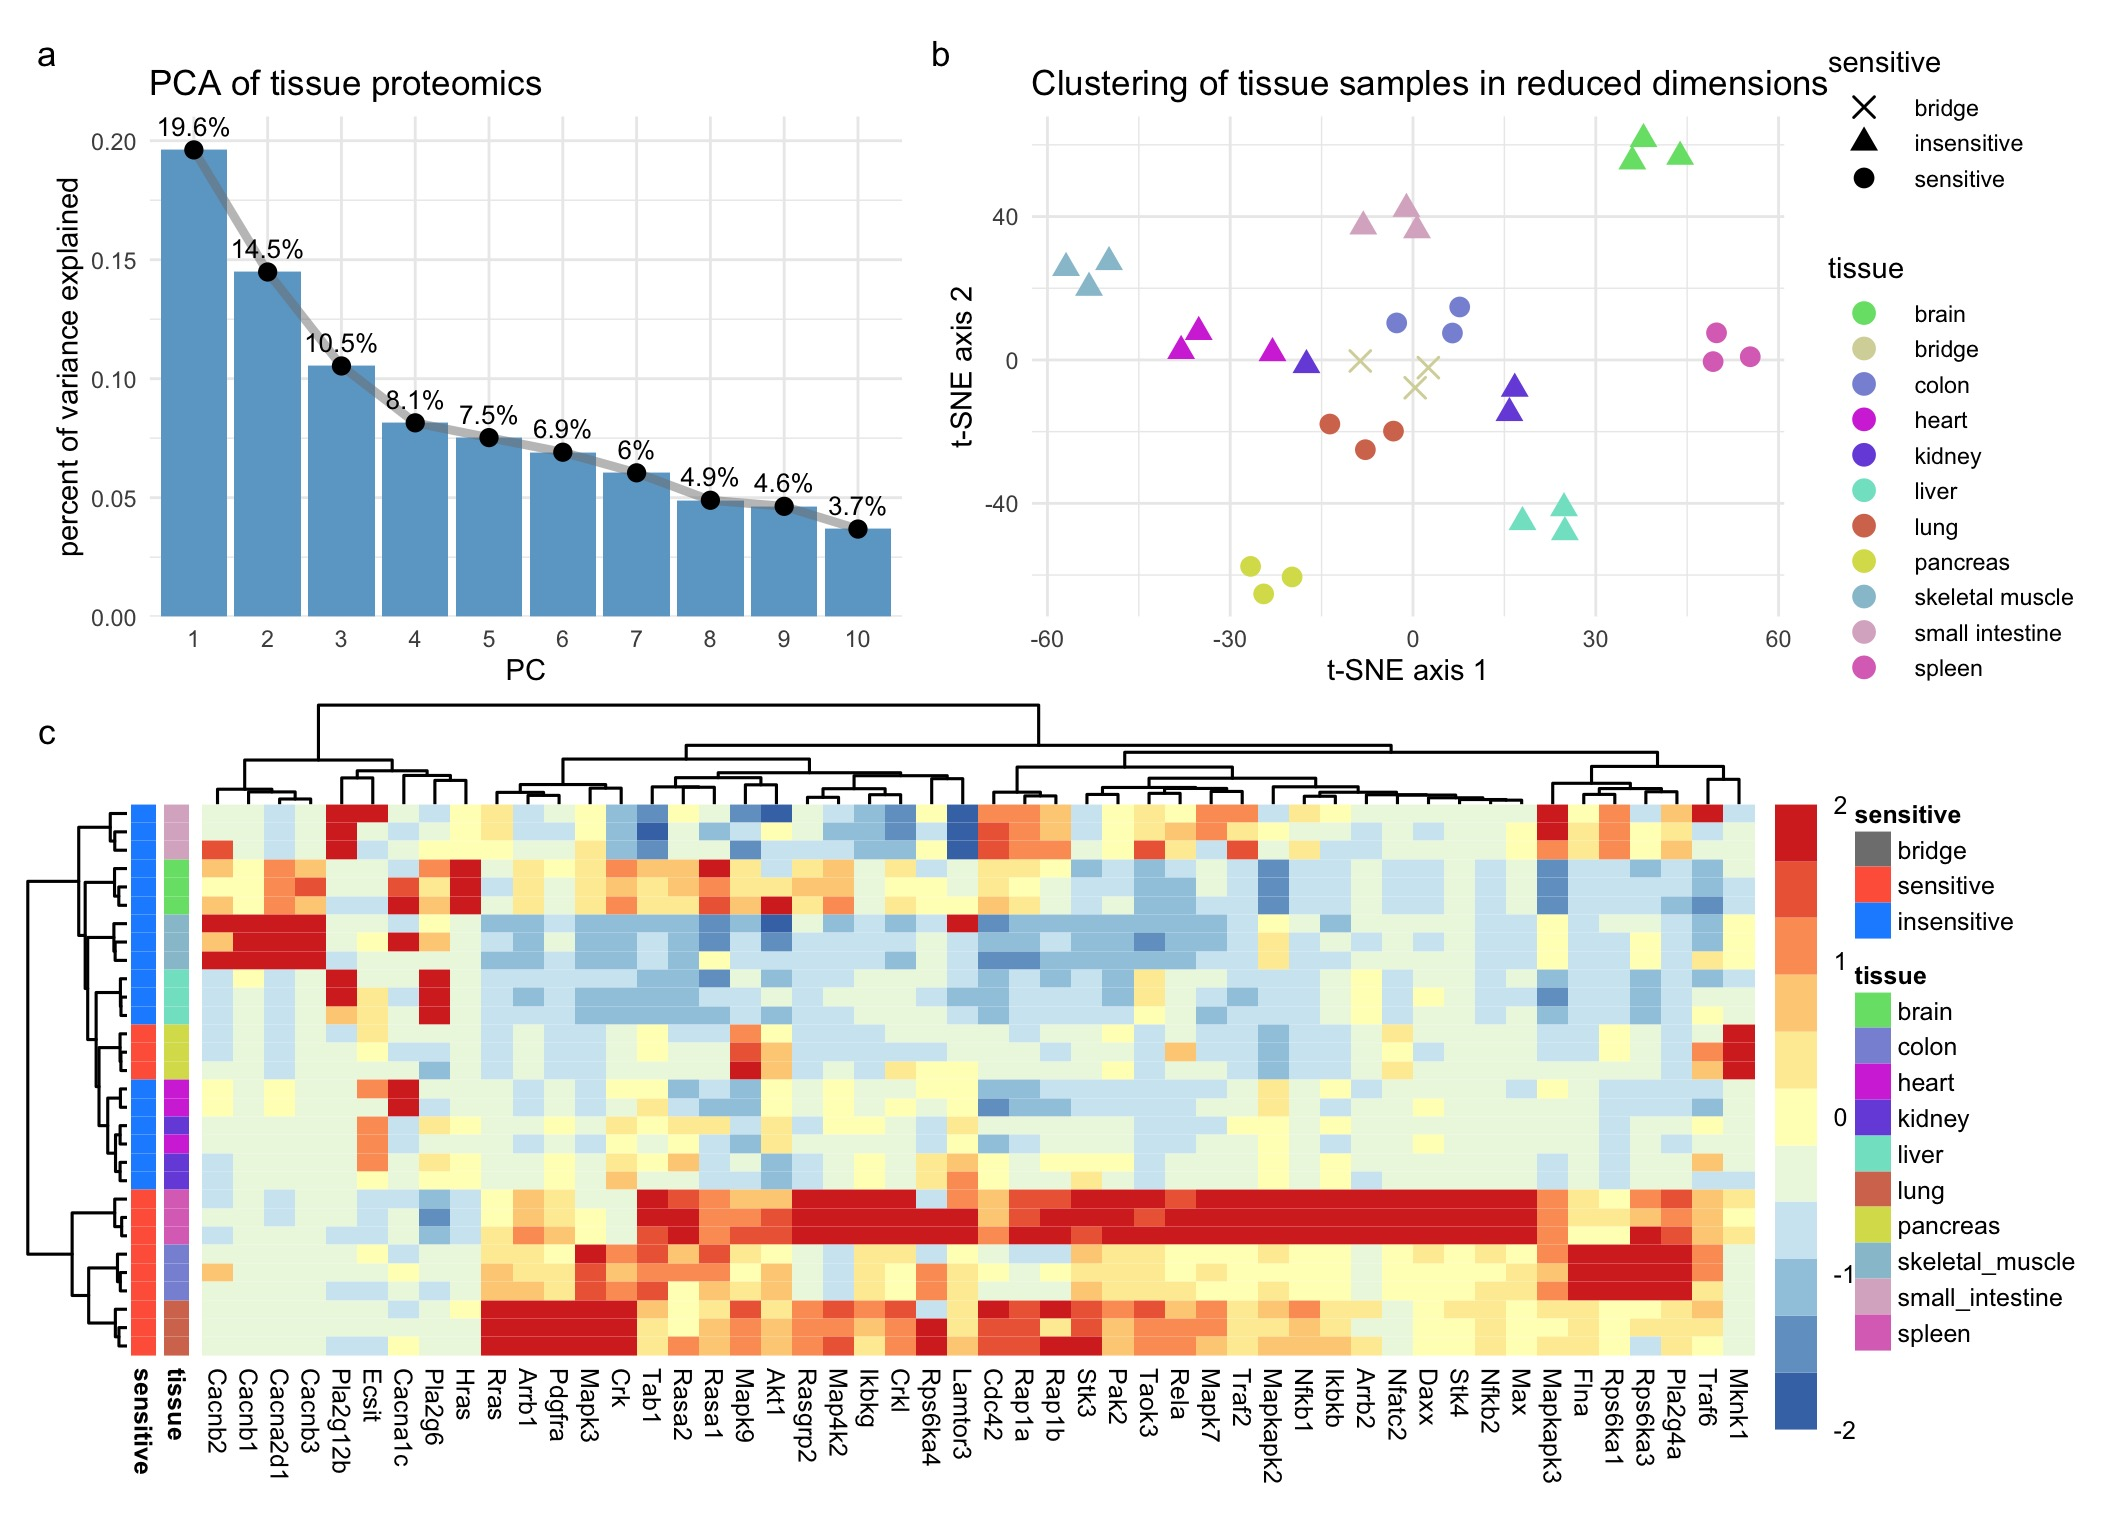
\includegraphics[width=180mm]{figures/aim2/proteomics-eda_figure.jpeg}
\caption{
    \textbf{The proteomics data cluster by tissue-type, not \KRAS{}-sensitivity.}
    \textbf{a.} The variance explained by the first ten principle components (PC) of the proteomics data.
    \textbf{b.} t-SNE applied to the new coordinates from PCA. Each point is colored according to the tissue and indicated to be \KRAS{}-sensitive or -insensitive by a circle or triangle, respectively. The bridge channels are indicated by "x"-marks.
    \textbf{c.} A heatmap of the 50 proteins with the strongest differences between sensitive and insensitive tissues (Student's \emph{t}-test, selected by p-value). Each column is a protein and each row is a tissue sample with the tissue and \KRAS{} sensitivity labeled by the column annotation.
}
\label{fig:proteomics-eda}
\end{figure}


%%%%%%%%%%%%%%%%%%%%%%%%%%%%%%%%%%%%%%%%%%%
% Aim 2.3
%%%%%%%%%%%%%%%%%%%%%%%%%%%%%%%%%%%%%%%%%%%

\subsection*{Aim 2.3. Identify recurring events in insensitive tissues with oncogenic \KRAS{} mutations.}

\subsubsection*{Approach}

Though the experimental evidence suggests that some tissues are not susceptible to hyperactive \kras{} signaling, there are still tumors from these locations that possess a mutation at a \KRAS{} hotspot.
While Aim 2.2 proposes to identify the differences between \KRAS{}-sensitive and insensitive tissues in homeostasis, this Aim approaches the question from the opposing direction: "What allowed \KRAS{} to drive these cancers in normally insensitive tissues?"

First, we will determine if these mutations were likely to have driven the cancer by measuring their allele-fraction in the sequencing data.
If the mutation to \KRAS{} was found in a small proportion of the sequencing reads that covered the \KRAS{} locus, then it was less likely to have driven tumor progression and was instead a passenger mutation.
In addition, if the data are available, we can analyze RNA and/or protein expression to ensure that the hyperactive allele was expressed.

If we find that the \KRAS{} mutations were likely to have acted as drivers in tumors originating in insensitive tumors, the we will proceed with characterizing recurrent genetic co-alterations.
This would include a comutation analysis similar to that described in Aim 1.2 to identify genes that tend to comutate with \KRAS{}.
Also, because the loss of tumor suppressor genes is important to the progression of \KRAS{}-driven cancers (e.g. the loss of \emph{APC} in COAD, \emph{STK11} and \emph{KEAP1} in LUAD, and \emph{CDKN2A} in PAAD), we will analyze the co-occurrence of copy number alterations (CNA) to known tumor suppressors.

Finally, we will use the conclusions from this analysis of human data to help understand the models in Aim 2.2.
As the models are looking for differences between multiple organs, it will be difficult to tell what is distinct due to tissue-specific functions and what is relevant to \KRAS{} sensitivity.
Thus, knowing what permitted an insensitive tissue to be transformed by a \KRAS{} mutation in human tumors will help interpret the findings from Aim 2.2.

\subsubsection*{Pitfalls and alternative approaches}

As noted in Aim 2.1, the sparsity of \KRAS{}-mutants tumors from \KRAS{}-insensitive tissues will be a limiting factor.
It will introduce a limit on the power of the analysis to detect more rare comutation events.

\subsubsection*{Preliminary data}

So far, I am still collecting and preparing data for analyses.
An overview of the number of tumor samples and how many have \KRAS{} mutations were displayed in Aim 2.1.

\subsection*{Vinay's notes on Aim 2}

{\color{red} test...

\begin{enumerate}
\item For aim 2.1, I think you should also explore the 
\end{enumerate}

}

\section{Aim 3. Assess the impact of PRC2 dysregulation on the tissue-specificity of cancer driver genes.}

\subsection*{Rationale}

As explained by Haigis \emph{et al.} in \cite{Haigis2019}, substantial evidence has lead us to hypothesize that the potential for a gene to drive cancer is predominately determined by the preexisting state of the cell and tissue microenvironment.
This state is determined by the epigenetic structure established over the development of the tissue.
By regulating gene expression, epigenetics establishes the transcriptome and proteome, defining the cellular signaling network.
Only the disruption to specific genes and proteins are oncogenic within the context of this network, thus defining the tissue-specificity of cancer driver genes.

PRC2 is responsible for maintaining gene silencing by methylating H3K27, and its activity is often ascribed to maintaining a cell's functional identity \cite{Comet2016MaintainingCancer., Laugesen2019a}.
Because the genes comprising this protein complex are frequently mutated or dysregulated (via changes in expression or gene copy number) in cancer \cite{Wassef2017, Comet2016MaintainingCancer.}, we propose it as a system through which to investigate the impact of the epigenome on tissue-specificity of cancer drivers.
\textbf{We hypothesize that the dysregulation of PRC2 methylation alters the state of a cell, and consequently alters the oncogenic potential of cancer driver genes.}

For this study, we will use data from a cancer type with a large number of sequenced samples and a high frequency of PRC2 mutations.
From a cursory inspection of The Cancer Genome Atlas (Figure \ref{fig:num-samples-prc2}), we propose using ovarian, uterine, breast, or skin cancer, though we will also account for data from other large consortia (such as the Pan-Cancer Analysis of Whole Genomes).

\begin{figure}[ht]
\centering
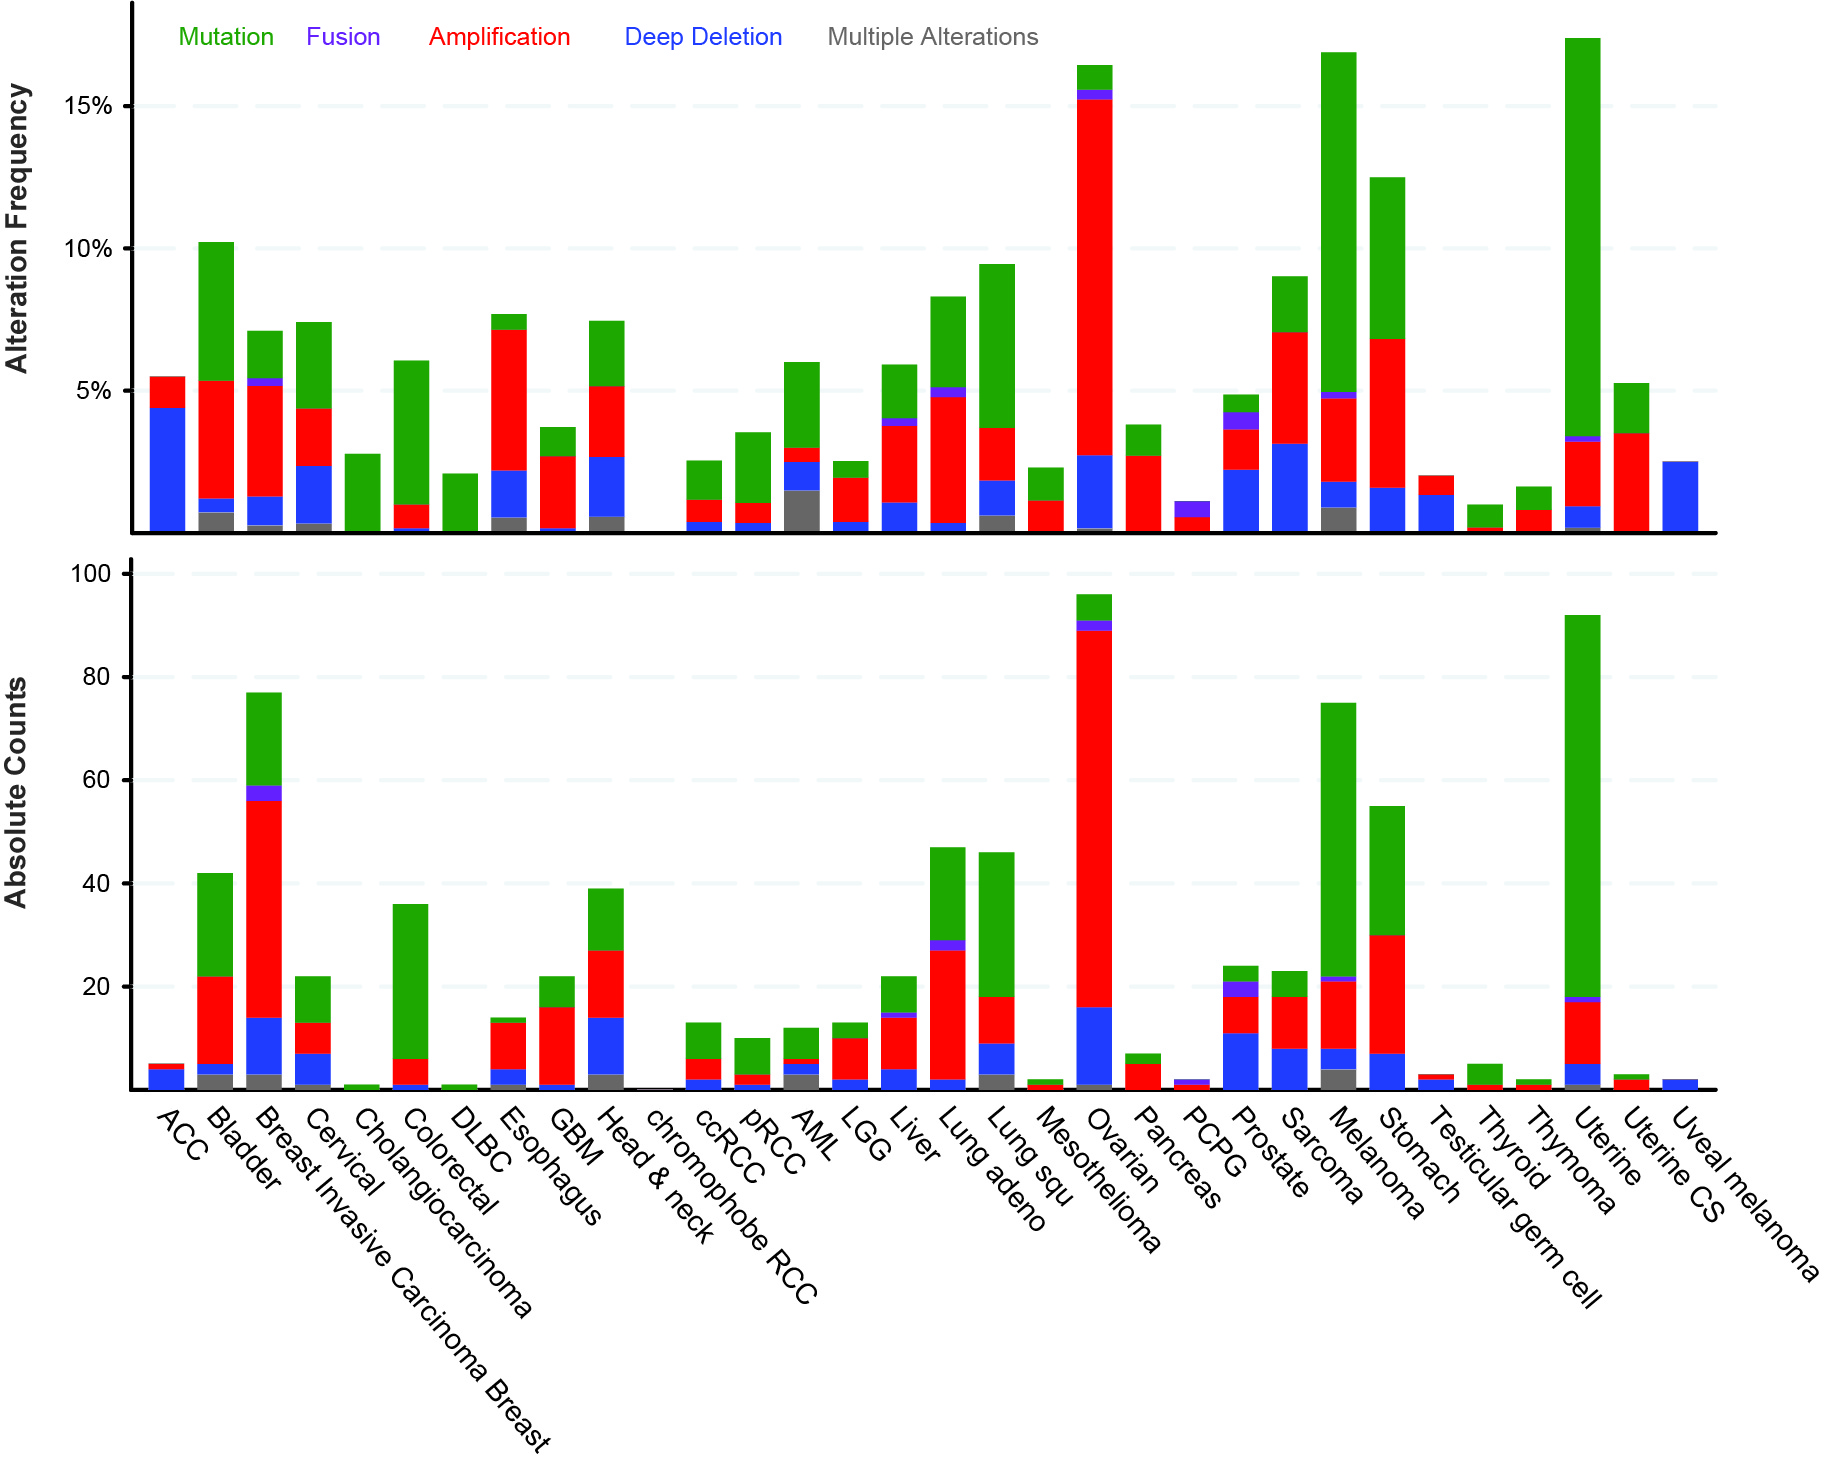
\includegraphics[width=155mm]{figures/aim3/FIG_number-of-samples.jpg}
\caption{
    \textbf{The frequency of alteration of PRC2 in different cancer types.}
    The frequency of alteration of PRC2 (top) and number of samples with altered PRC2 (bottom) in The Cancer Genome Atlas. Somatic mutations to \emph{EZH1}, \emph{EZH2}, \emph{EED}, and \emph{SUZ12} were included. \href{https://www.cbioportal.org/results/cancerTypesSummary?Action=Submit&RPPA_SCORE_THRESHOLD=2.0&Z_SCORE_THRESHOLD=2.0&cancer_study_list=laml_tcga_pan_can_atlas_2018\%2Cacc_tcga_pan_can_atlas_2018\%2Cblca_tcga_pan_can_atlas_2018\%2Clgg_tcga_pan_can_atlas_2018\%2Cbrca_tcga_pan_can_atlas_2018\%2Ccesc_tcga_pan_can_atlas_2018\%2Cchol_tcga_pan_can_atlas_2018\%2Ccoadread_tcga_pan_can_atlas_2018\%2Cdlbc_tcga_pan_can_atlas_2018\%2Cesca_tcga_pan_can_atlas_2018\%2Cgbm_tcga_pan_can_atlas_2018\%2Chnsc_tcga_pan_can_atlas_2018\%2Ckich_tcga_pan_can_atlas_2018\%2Ckirc_tcga_pan_can_atlas_2018\%2Ckirp_tcga_pan_can_atlas_2018\%2Clihc_tcga_pan_can_atlas_2018\%2Cluad_tcga_pan_can_atlas_2018\%2Clusc_tcga_pan_can_atlas_2018\%2Cmeso_tcga_pan_can_atlas_2018\%2Cov_tcga_pan_can_atlas_2018\%2Cpaad_tcga_pan_can_atlas_2018\%2Cpcpg_tcga_pan_can_atlas_2018\%2Cprad_tcga_pan_can_atlas_2018\%2Csarc_tcga_pan_can_atlas_2018\%2Cskcm_tcga_pan_can_atlas_2018\%2Cstad_tcga_pan_can_atlas_2018\%2Ctgct_tcga_pan_can_atlas_2018\%2Cthym_tcga_pan_can_atlas_2018\%2Cthca_tcga_pan_can_atlas_2018\%2Cucs_tcga_pan_can_atlas_2018\%2Cucec_tcga_pan_can_atlas_2018\%2Cuvm_tcga_pan_can_atlas_2018&case_set_id=all&data_priority=0&gene_list=EZH2\%252C\%2520EZH1\%252CEED\%252CSUZ12&geneset_list=\%20&profileFilter=0&tab_index=tab_visualize}{cBioPortal} was used to collect and visualize the data \cite{Cerami2012, Gao2013}.
}
\label{fig:num-samples-prc2}
\end{figure}

%%%%%%%%%%%%%%%%%%%%%%%%%%%%%%%%%%%%%%%%%%%
% Aim 3.1
%%%%%%%%%%%%%%%%%%%%%%%%%%%%%%%%%%%%%%%%%%%

\subsection*{Aim 3.1. Identify differences in mutations associated with dysregulated PRC2.}


\subsubsection*{Approach}

If the epigenetic state of a cell determines its susceptibility to different cancer driver genes, then we expect to find different genes mutated when PRC2 function is altered.
To this end, we will identify genes that are more or less frequently mutated in PRC2-dysfunctional tumors compared to those with normal PRC2. 
Of these genes, the properties of the known oncogenes, along with a functional enrichment analysis of the others, will describe the distinct changes induced by PRC2-mediated epigenetic changes.

We can identify more complex rearrangements of the cellular signaling structure by identifying new modules of comutating or mutually-exclusive genes in PRC2-dysfunctional tumors using existing computational methods \cite{Miller2011, Vandin2012, Ciriello2012, Jia2014, Zhang2014c, Ahmed2015, Kim2015, Leiserson2015, Babur2015, Leiserson2015b, Dao2017, Leiserson2016, Cho2016a, Reyna2018, Zhang2018e, Bokhari2020QuaDMutNetEx:Frequency.}.
Genes often comutate because the events cooperate in driving cancer or are mutually-exclusive because they are redundant or due to synthetic lethal \cite{Kaelin2005} or collateral lethal \cite{Muller2015} interactions.
Therefore, comutation or mutually exclusive interactions that are unique or lost in PRC2-mutant tumors would suggest that the epigenetic alterations have greatly influenced the signaling pathways.

It is known that chromatin structure plays a substantial role in the distribution of mutations along the chromosomes \cite{Schuster-Bockler2012, Polak2015, Gonzalez-Perez2019}.
Thus, the mutational patterns identified in the above analyses could be due, in part, to changes in their proximity in 3D-space or degree of chromosomal compaction elicited by altered PRC2 behaviour.
We will include this in the analysis by identifying "spatial comutation hotspots" \cite{Shi2016ChromatinGenes}, thus linking dysregulated PRC2-mediated chromatin organization to the increased rates of mutation or changes in comutation and mutually exclusive modules.
We will use the the epigenomic map created by the Roadmap Consortium \cite{Polak2015} as a reference for the normal chromatin state.

Overall, the analyses proposed above represent a comprehensive characterization of changes to cancer progression induced by aberrant PRC2 epigenetic regulation.


\subsubsection*{Pitfalls and alternative approaches}

As PRC2 is a protein complex with multiple subtypes thought to modify its recruitment and enzymatic function \cite{Wassef2017, Holoch2017, Kasinath2018, Laugesen2019a}, we expect different mutations of the subunits of PRC2 to have different impacts.
All of the genes encoding the core PRC2 subunits have known loss-of-function alterations and some, particularly \emph{EZH2}, have known gain-of-function alterations \cite{Comet2016MaintainingCancer.}.
Therefore, a careful survey of the RNA expression, copy number, and missense mutations to the genes comprising PRC2 will be conducted prior to the above analyses.

Since we want to prescribe altered rates of mutation to changes in PRC2 activity, knowing the timing of the events may be important.
The process of ordering mutations acquired during tumorigensis is best accomplished using single-cell analyses.
Thus, it may be possible to determine the timing of events in single-cell sequencing data of tumors where the component genes of PRC2 contained somatic mutations.
Further investigation is needed to fully understand if the analysis of single-cell genome sequencing is a viable means of determining the order of events identified in the previous analyses.



%%%%%%%%%%%%%%%%%%%%%%%%%%%%%%%%%%%%%%%%%%%
% Aim 3.2
%%%%%%%%%%%%%%%%%%%%%%%%%%%%%%%%%%%%%%%%%%%

\subsection*{Aim 3.2. Determine genetic dependencies associated with aberrant PRC2 function.}


\subsubsection*{Approach}

As dysregulated PRC2 alters the cellular signaling context of a tumor, we expect distinct dependencies on cellular processes to arise \cite{Kim2015SWI/SNF-mutantEZH2., Fillmore2015EZH2Inhibitors., Serresi2016PolycombCancer., Serresi2018Ezh2Vulnerabilities., Chen2018TargetingMedicine.}.
Thus, we will again utilize the Cancer Dependency Map Project's CRISPR-Cas9 knockout screen \cite{Tsherniak2017, Meyers2017} to identify genes that are differentially dependent in PRC2-mutant cancer cell lines.
As before, we will create a linear model for each gene that will use the RNA-expression of the gene, its mutational status, and the status of PRC2 to predict the effect of knocking-out the gene on the cell's proliferation.
We will also build models that include binary indicators for the common oncogenes and tumor suppressor genes found in each cancer type.
These models will be compared to estimate the importance of altered PRC2 activity on the dependency on each gene.
Further information from the genes found to have differential dependence per the activity of PRC2 will be gathered by finding which cellular processes are enriched in the results.

As we are interested in the potency of oncogenes in the presence of normal and altered PRC2 activity, we will also build specific models for the dependence of known oncogenes and those with increased or reduced rates of mutation in PRC2-mutant tumors (from Aim 3.1) that include an interaction term between the oncogene and PRC2 activity.
These terms will indicate whether there is an effect of a cell having a mutation to the oncogene and dysregulated PRC2 on the dependency of the cell on the oncogene.
Comparing these models to those without the interaction term will indicate if the interaction was important.


\subsubsection*{Pitfalls and alternative approaches}

An alternative approach to building a model for each individual gene as proposed above would be to build models for entire pathways or cellular functions instead.
This would recognize instances where the PRC2 dysregulation has caused the dependency on a group of genes to change, but where each cell line has different genes in the set that have altered dependency or the dependency is spread amongst multiple genes.
One foreseeable difficulty will be finding a single metric to summarise the dependency score for an entire pathway for each cell line.
One option would be to use Gene Set Variation Analysis \cite{Hanzelmann2013} or a related method \cite{Barbie2009, Lee2008InferringClassification., Tomfohr2005PathwayDecomposition., Jung2011ComparisonGenes.} to transform the gene level data into a pathway level enrichment score for each cell line.


% {\color{red} 
% Vinay's comments
% \begin{enumerate}
%     \item Why is "Rationale" incomplete? Are you filling this in?
%     \item For the spatial determinants -- you could also consider whether the co-mutated regions also exist within regions marked with specific chromatin modifications in normal tissue. Polak and colleagues checked for such context when inferring cell-of-origin. Additionally, if you are doing a co-mutation or mutational process study, you will need to control for local sequence composition
%     \item The rationale for why PRC2-activated would be mutated more in PRC2-mutant tumors is unclear, unless you already expect that open/closed chromatin in PRC2-mutant tumors have different mutational rates. 
% \end{enumerate}
% }


\chapter{Conclusion}

Recognizing the tissue-specificity of cancer driver genes is essential to precision medicine.
Indeed, the role of an individual oncogene is context dependent and, thus, distinct in each cancer type.
The studies described here investigate tissue-specificity via two mechanisms.
The first aims to characterize the properties of a single gene, \KRAS{}, in multiple contexts including in tissues where it is a potent oncogene and in tissues with built-in resistance.
The second mechanism studies the causes of a change to the cellular context via epigenetic dysregulation.
These two approaches represent a multi-faceted and unique analysis of a phenomenon critical to our understanding of cancer.


%%%%%%%%%%%%%%%%%%%%%%%%%%%%%%%%%%%%%%%%%%%
% Appendices
%%%%%%%%%%%%%%%%%%%%%%%%%%%%%%%%%%%%%%%%%%%
% \appendix

% \chapter{An example of an appendix}
This is what an appendix looks like!

% \label{sec:session}
\chapter{Session Protocol}
%% This shows appendix shows how to attach a file to the appendix.
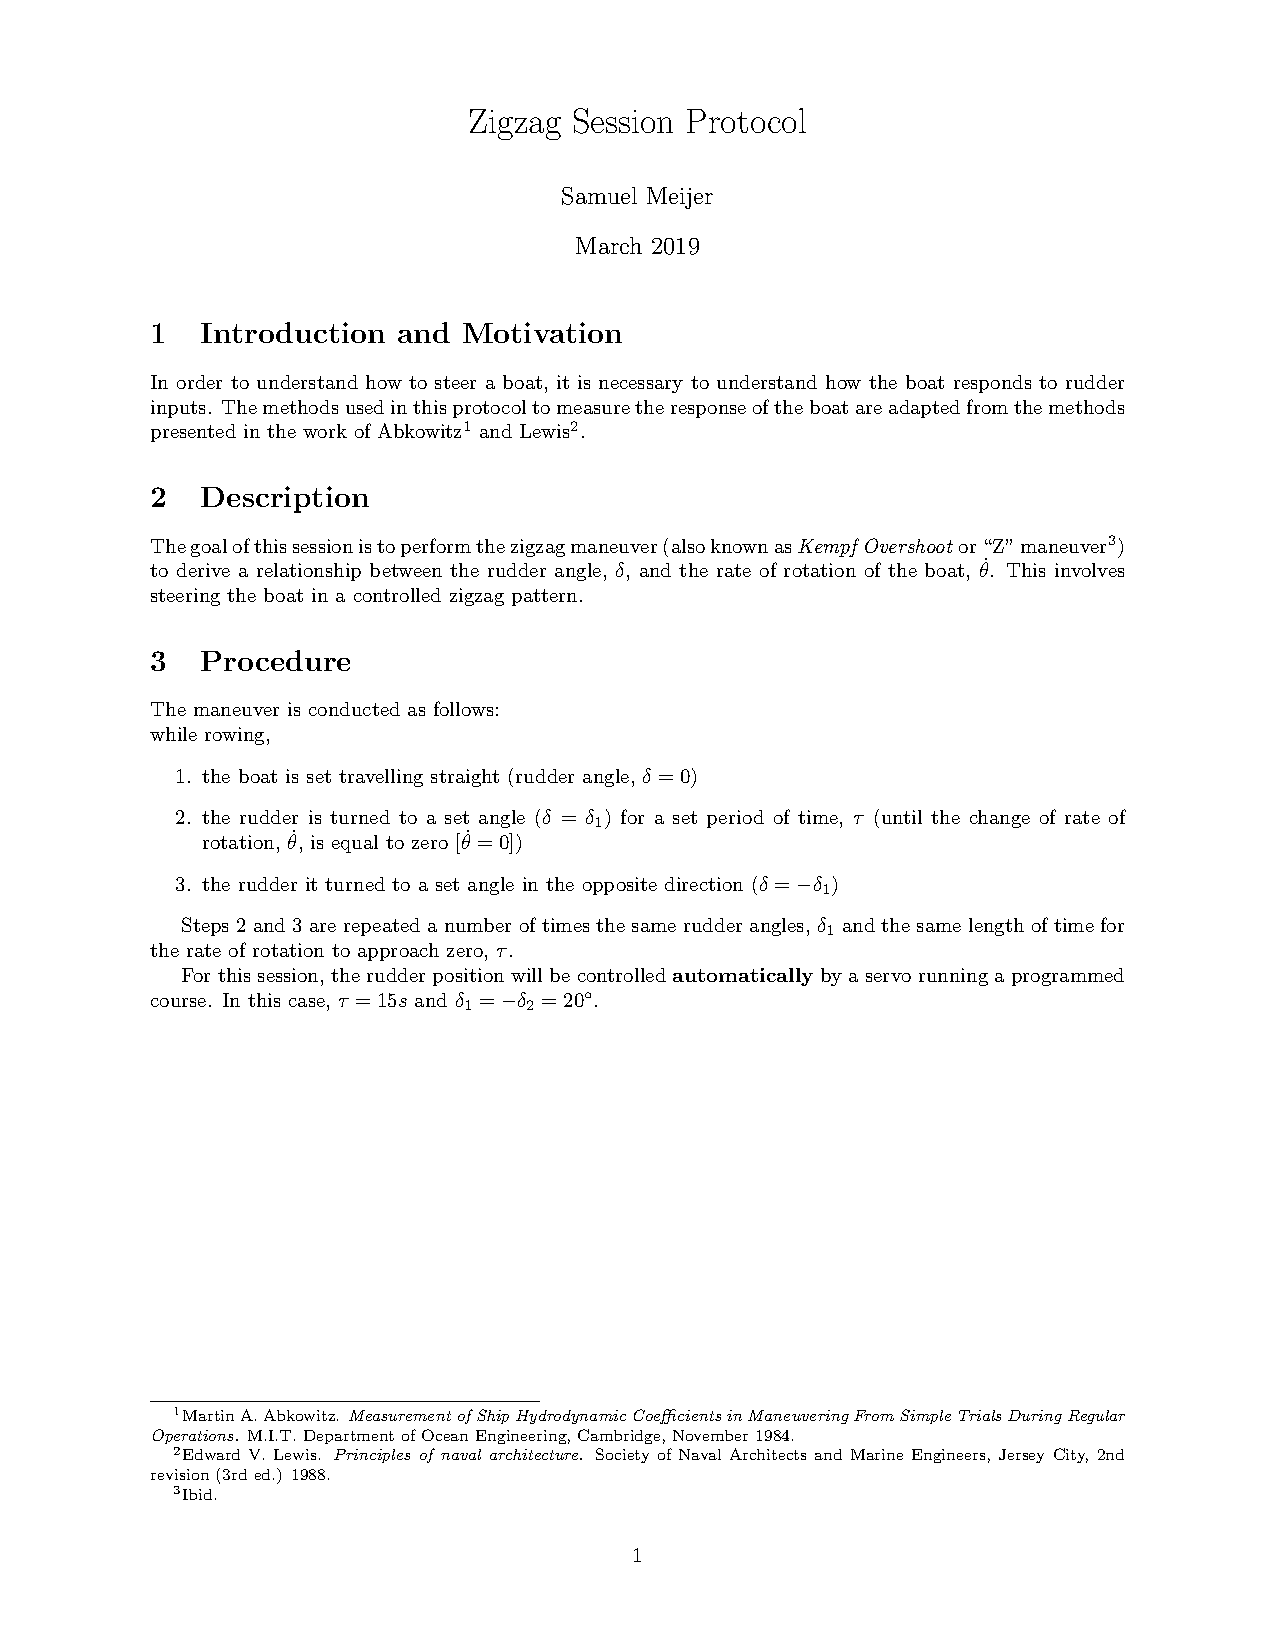
\includepdf[]{appendices/Session_Protocol-3.pdf}


% \chapter{Software}\label{app:software}
 %% You may want to include some code in your thesis. I found this method online, and would recommend you do the same... See preamble/arduinoLanguage.tex for the file that makes it look nice.
\begin{lstlisting}[language=Arduino]  
#include <Wire.h>
#include <Adafruit_Sensor.h>
#include <Adafruit_BNO055.h>
#include <utility/imumaths.h>
#include <Adafruit_GPS.h>
#include <SPI.h>
#include <SD.h>
#include <Servo.h>
#include <math.h>
#include "Filter.h"

/* This driver reads raw data from the BNO055, Potentiometer and GPS

   Connections for ADALOGGER
   ===========

   Potentiometer
   _____________
   Connect one side to VCC
   Connect other to common ground
   Connect Middle to A0

   GPS
   _____________
   Connect VIN to VCC
   Connect GROUND to common ground
   Connect GPS TX to RX1 (D0)
   Connect GPS RX to TX1 (D1)

*/

/*********************************************/
/*BNO055 (orientation) setup, variables and def'n*/
/*********************************************/
// Sample delay
const float SAMPLERATE = 10;
// Setup for the differentiation variables
double psierror = 0;
double dt = 0;
double dpsierror_dt = 0;
double previouspsierror = 0;

\end{lstlisting}

%%%%%%%%%%%%%%%%%%%%%%%%%%%%%%%%%%%%%%%%%%%
% Bibliography
%%%%%%%%%%%%%%%%%%%%%%%%%%%%%%%%%%%%%%%%%%%

\bibliographystyle{unsrt}
\bibliography{reference_files/references}{}


\end{document}